\documentclass[12pt]{article}

\usepackage[a4paper,top=2cm,bottom=2cm,left=2cm,right=2cm,marginparwidth=1.5cm]{geometry}
\usepackage{graphicx}
\usepackage{amssymb}
\usepackage{epstopdf}
\usepackage[german]{babel}
\usepackage[utf8]{inputenc}
\usepackage{pdfpages}
\usepackage{fancyhdr}
\DeclareGraphicsRule{.tif}{png}{.png}{`convert #1 `dirname #1`/`basename #1 .tif`.png}

%neu Adrika
\usepackage{tabularx}
\usepackage{float}
\usepackage{caption} 


\title{Bericht}
\author{Alisa Pesteritz, Saliha Altan, Wiktoria Cholewa, \\ 
	Dominik Falk, Andreas Kasarinow, Johanna Kleidorfer, \\
	Adrika Narasimhan, Rosina Röckseisen}

\begin{document}

\newpage
\maketitle

\newpage
\pagestyle{fancy}
\fancyhead{}
\fancyhead[L]{Alle}
\section{Einleitung}
\label{einleitung}

\section{Arbeitseinteilung (oder sowas)}
\label{arbeitseinteilung}
% TODO: Wer hat was gemacht und warum?
% Datenfluss (von Johanna) einfügen? (oder zumindest beschreiben?)

% ----------------------------------------------------------------------------------------------
\newpage
\pagestyle{fancy}
\fancyhead{}
\fancyhead[L]{Alisa}
\section{Pathways und Dateneinlesen}
\label{pathways}

% ----------------------------------------------------------------------------------------------
\newpage
\pagestyle{fancy}
\fancyhead{}
\fancyhead[L]{Rosina \& Wiki}
\section{Normalisierung}
\label{normalisierung}


\section{Clusteranalyse}
\label{clusteranalyse}
% TODO: theoretische Erklärung des Algorithmus

\subsection{Single Linkage}
\label{single-linkage}

\subsection{Average Linkage}
\label{average-linkage}

\subsection{Complete Linkage}
\label{complete-linkage}

% ----------------------------------------------------------------------------------------------
\newpage
\pagestyle{fancy}
\fancyhead{}
\fancyhead[L]{Saliha \& Domi}
\section{Visualisierung}
\label{visualisierung}

\subsection{Heatmap}
\label{heatmap}

\subsection{Dendrogramm}
\label{dendrogramm}

% ----------------------------------------------------------------------------------------------
\newpage
\pagestyle{fancy}
\fancyhead{}
\fancyhead[L]{Adrika}

\section{GUI}
\label{gui}

\subsection{Arbeitsverteilung}
\label{GUI-arbeitsverteilung}
Der Bereich der Graphical User Interfaces (GUIs) unterteilt sich in verschiedene Abschnitte. Vor allem sind die wichtigsten jeweils die Erstellung des Frontend-User-Interfaces, die Verbindung mit Back-end-Funktionen, PDF-Export, Sichern von Einstellungen, Einlesen von Datensätzen und Verschönerung des Layouts. Die folgende Tabelle zeigt die Arbeitsverteilung des Teams GUI.

\begin{table}[h]
\centering
	\begin{tabular}{l|l|l}
		Aufgabe & Zuständig & Arbeitsaufwand \\ 
		\hline
		Erste Visualisierung des Dashboards             & Adrika    & 2 Stunden        \\
		Verbindung von allen Backend-Funktionen       & Adrika  &  27 Stunden      \\ 
        Sichern von Einstellungen & Adrika & 4 Stunden \\
		Fehler Meldungen              & Adrika    & 3 Stunden        \\ 
        Layout verschönern & Adrika & 4.75 Stunden \\
        Alle UI-Elemente implementieren & Adrika & 15 Stunden \\
        Bericht schreiben & Adrika & 9.5 Stunden \\
        Besprechungen & Adrika & 25 Stunden \\ 
        Erstellung von Folien & Adrika & 3 Stunden 

        
	\end{tabular}
\end{table}

\subsection{Verwendete Pakete}
Die folgende Tabelle gibt eine Zusammenfassung aller verwendeten Pakete innerhalb von Shiny, die sehr wichtig sind, um ein Dashboard zu erstellen. 

\begin{table}[h]
\centering
	\begin{tabular}{|l|p{14cm}|}
        \hline
		Paket & Aufgabe \\ 
		\hline
		shiny & R-Paket, mit dem man Web-Apps und Dashboards erstellen kann \cite{shiny}\\
        \hline
        dipsaus & Add-on-Paket für Shiny, um praktische Funktionen und Verbesserungen hinzuzufügen \cite{dipsaus}\\
        \hline
        shinydashboard & wichtig für die Erstellung eines einfachen Dashboard mit Header, Sidebar, und Body \\
        \hline
        shinyFeedback & wichtig für die Anzeige von Warnungen, oder generelle User-friendly Nachrichten \\
        \hline
        shinyjs & wichtig für die Verwendung von nützlichen JavaScript-Operationen \cite{shinyjs}\\
        \hline
        bslib & wichtig für die Erstellung von custom bootstrapping-themes, was es einfacher macht Shiny-Apps zu stylen \cite{bslib}\\
        \hline
        bsicons & Paket, wichtig für die Verwendung von Bootstrap Icons in Shiny \cite{bsicons}\\
        \hline
        shinyBS & bietet extra interaktive UI-Komponenten für Shiny-Apps wie Modal Pop-ups zum Beispiel \cite{shinyBS} \\
        \hline

        
	\end{tabular}
\end{table}

\newpage
\subsection{Aufgaben}
\label{wichtigeAufgaben}

\subsubsection{Entwicklung der Benutzeroberfläche}

Zu Beginn des Projekts war es sehr wichtig, dass das Team GUI eine erste \textbf{Visualisierung des Dashboards} erstellte. Dieser Prototyp wurde mit Canva erstellt und lieferte einen ersten Einblick darin, wie das Dashboard aussehen sollte, damit es auf dieser Grundlage aufgebaut werden konnte. Dann wurde \textbf{R Shiny} verwendet, um diesen Prototyp zu einem echten Dashboard weiterzuentwickeln. Das war das Kernprogramm, um ein Dashboard für die Clusteranalyse zu entwickeln.

Mit dem \textbf{shinydashboard}-Paket war es möglich, ein leeres Dashboard mit Header, Sidebar und Body zu erstellen. Das war der grundlegende Aufbau des Projekts. Um die Benutzeroberfläche weiterzuentwickeln, war es am wichtigsten, verschiedene Tabs für unterschiedliche Nutzungen zu haben. Damit gab es eine Startseite, die die wertvollsten Informationen zu unseren Dashboards hatte, einen Datei-Hochladen-Tab, wobei der User eine CSV-Datei hochladen konnte und verschiedene Pathways auswählen durfte, einen Parameter-Auswahl-Tab zur Auswahl aller benötigten Parameter, um eine eindeutige und komplette Clusteranalyse durchzuführen, und am wichtigsten einen Visualisierungstabs, an welchem das Grafikpanel und die Dendrogramme erstellt wurden. 

Zusätzlich gibt es bei den UI-Elementen von Shiny mehrere \textbf{Control Widgets}, um User-Eingabe zu kontrollieren und zu verarbeiten \cite{ControlWidgets}. Als Erstes wurde die Pathways-Auswahl beim Dateihochladen erstellt. Weil es für einen User notwendig ist, mehrere Pathways auswählen zu können, wurde hier ein \textbf{SelectizeInput-Widget} verwendet, welches die Auswahl eines oder mehrerer Elemente aus einer Liste ermöglicht. Abbildung \ref{fig:pathways} zeigt ein Beispiel davon aus dem Dashboard. Daneben war bei der Parameter-Auswahl im Tab natürlich wichtig, dass der User die Möglichkeit hat, unterschiedliche Parameter auszuwählen, damit das Dashboard eine präzise und sinnvolle Clusteranalyse durchführen kann. Hierbei wurde eine Mischung aus \textbf{Radio-Buttons} und \textbf{Drop-down-Menü-Widgets} verwendet. Abbildung \ref{fig:parameter} zeigt, wie das Parameter-Auswahl-Tab am Ende aussieht. Bei der Clusterverfahrensauswahl, der Normalisierungsverfahrensauswahl und der Distanzmatrixauswahl wurden Drop-down-Menüs mit der Funktion \textbf{selectInput} angewendet. Bei der Farbpalettenauswahl war es aber sinnvoller, Radio-Buttons mit der Funktion \textbf{radioButtons} zu benutzen, weil es deutlich klarer und einfacher macht, Informationen über die in den Namen enthaltenen Farben umzusetzen.


\begin{center}
\begin{minipage}[t]{0.35\textwidth}
    \centering
    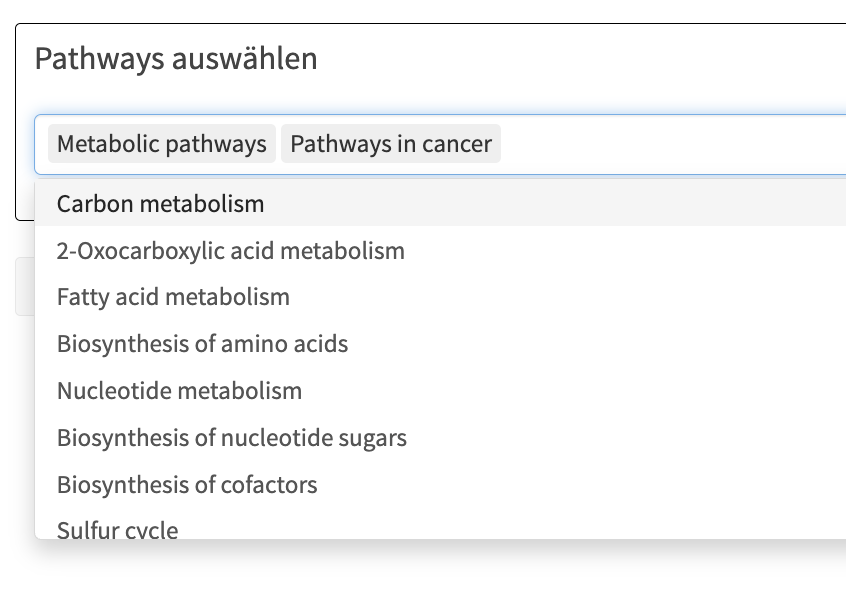
\includegraphics[width=\linewidth]{pathways.png}
    \captionof{figure}{Beispiel der Pathway-Auswahl}
    \label{fig:pathways}
\end{minipage}
\hfill
\begin{minipage}[t]{0.3\textwidth}
    \centering
    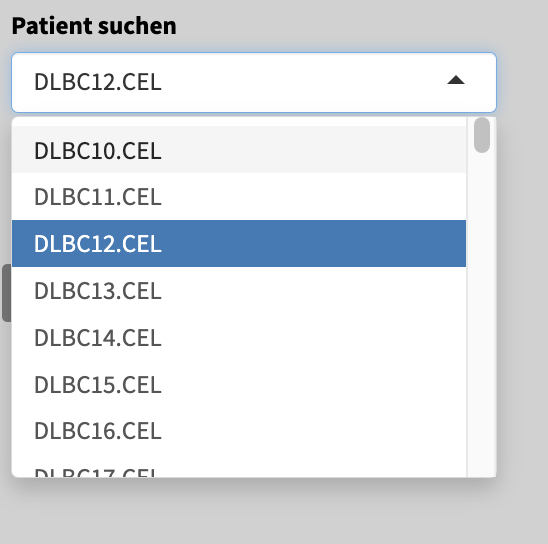
\includegraphics[width=\linewidth]{patientsuchen.png}
    \captionof{figure}{Beispiel der Patientensuche}
    \label{fig:patient}
\end{minipage}
\hfill
\begin{minipage}[t]{0.2\textwidth}
    \centering
    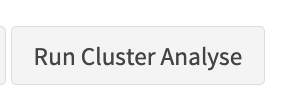
\includegraphics[width=\linewidth]{runButton.png}
    \captionof{figure}{Beispiel der Action Button}
    \label{fig:runButton}
\end{minipage}

\hfill
\begin{minipage}[t]{0.98\textwidth}
    \centering
    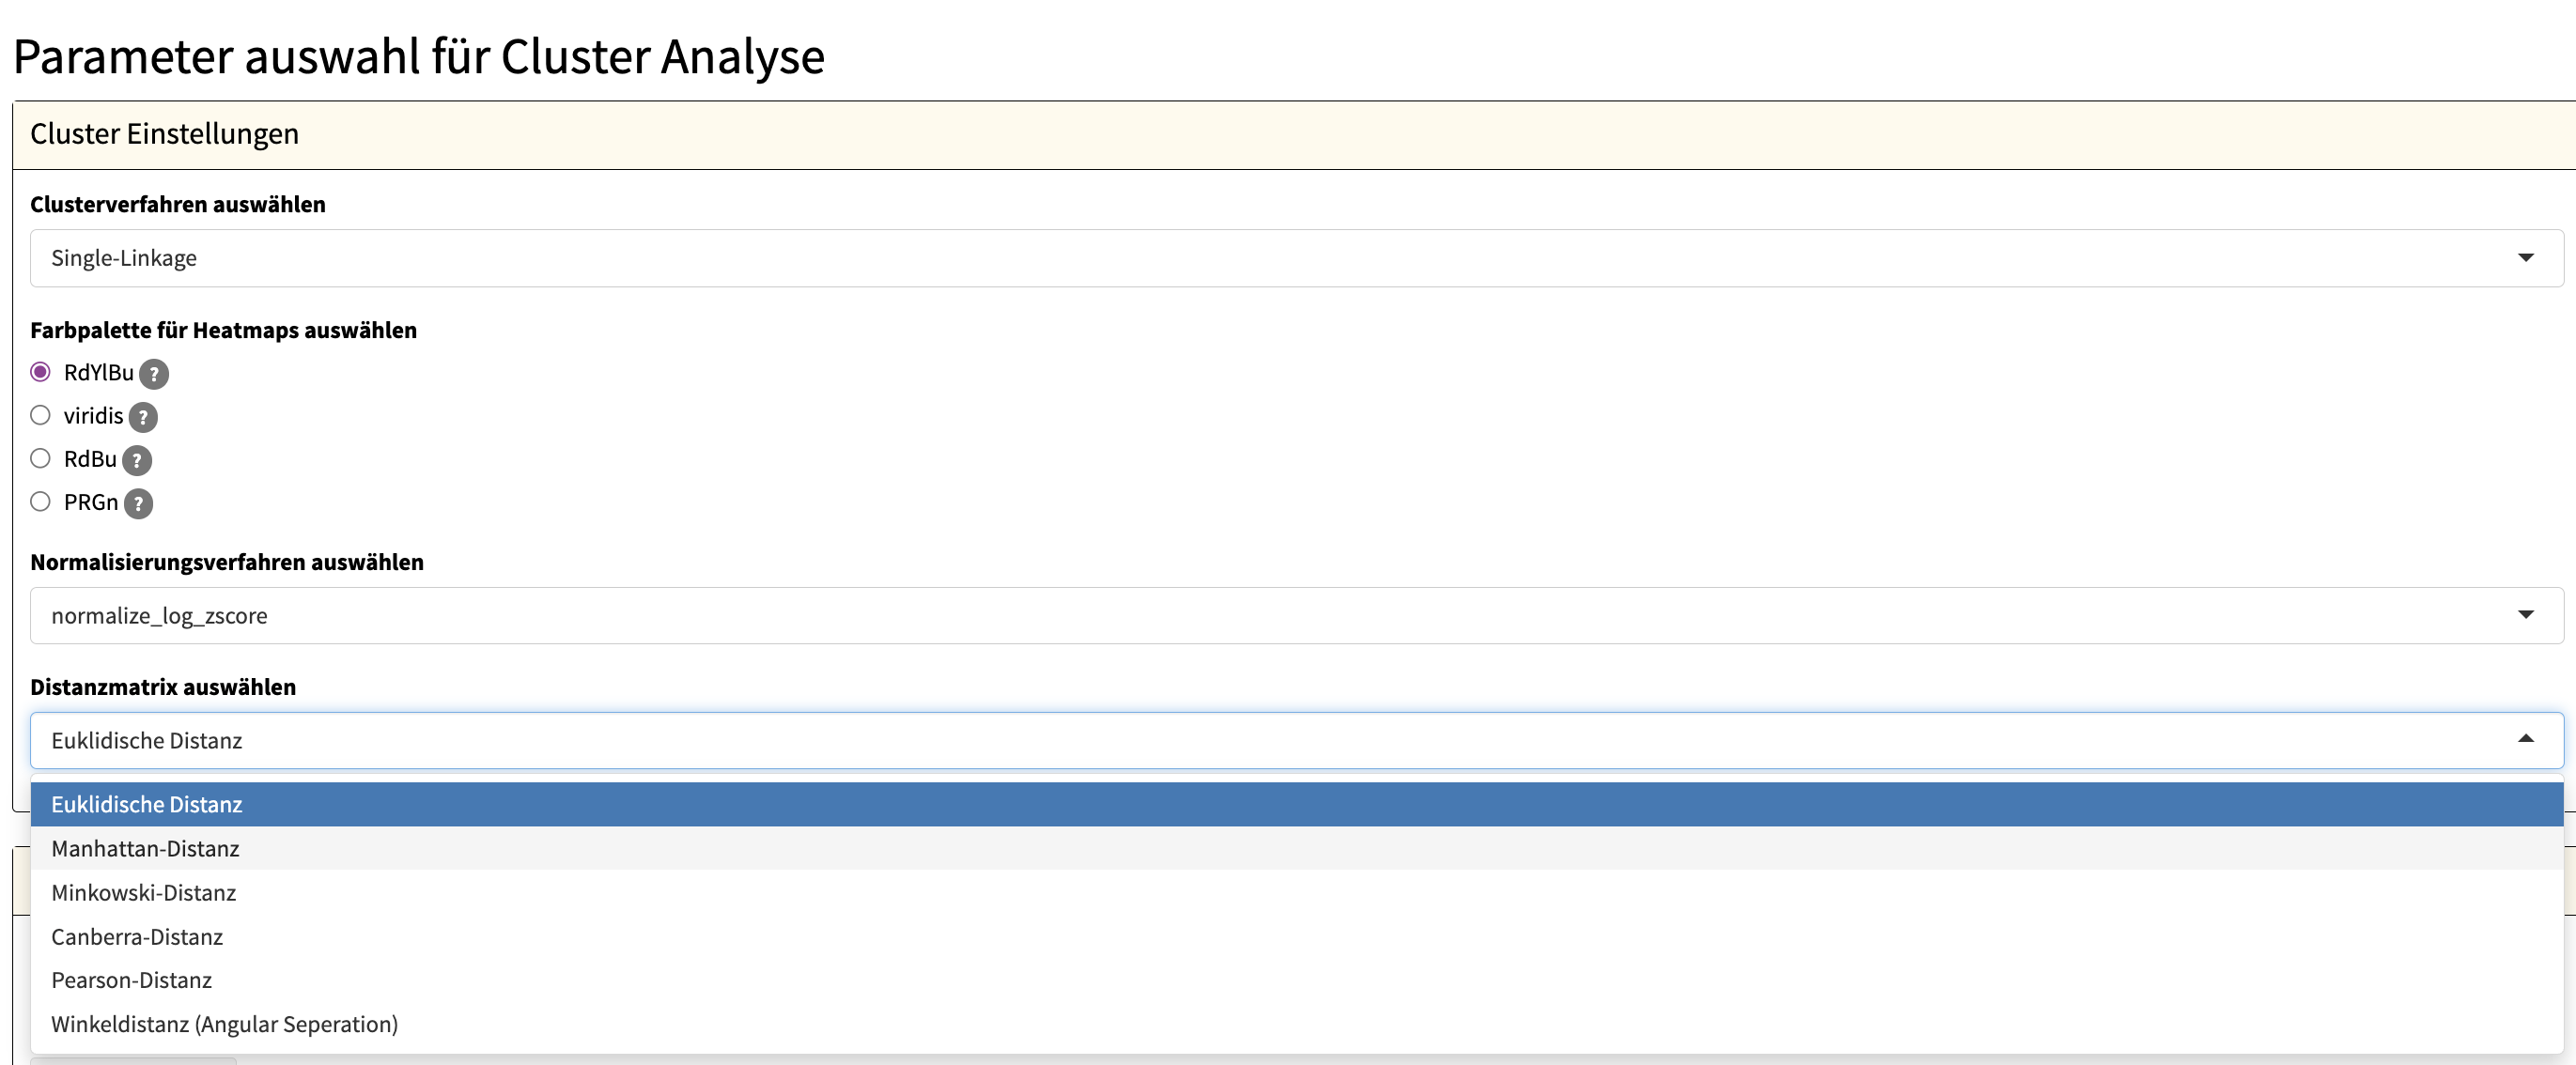
\includegraphics[width=\linewidth]{parameter.png}
    \captionof{figure}{Beispiel der Parameterauswahl}
    \label{fig:parameter}
\end{minipage}
\end{center}

Die gleichen Parameter wurden auch innerhalb der Sidebar beim Visualisierungs-Tab eingesetzt, damit es für den User einfacher ist, die Parameter direkt im gleichen Tab zu ändern. Jedoch war es wichtig, dass diese Parameter nur beim Visualisierungs-Tab angezeigt werden und nicht bei den anderen Tabs. Dafür wurde die \textbf{conditionalPanel}-Funktion eingesetzt, die ein Panel erstellt, das nur je nach dem Wert eines JavaScript-Ausdrucks angezeigt wird oder nicht. In diesem Fall musste es nur angezeigt werden, nachdem der User im Visualisierungs-Tab ankam. Für diese Funktion ist auch das shinyJS-Paket wichtig. Bei dem Tab wurde auch ein Suchfeld für Patienten eingebaut, wie auf der Abbildung \ref{fig:patient} zu sehen ist. Das Ziel dieser Parameter ermöglicht es dem Arzt, auch mit der selectizeInput-Funktion nach einem Patienten innerhalb der Grafikpanels zu suchen. Dies wurde auch dynamisch eingesetzt, damit es sich für jeden Datensatz an die Patienten dynamisch anpasst. 

Letztendlich wurden auch mehrere \textbf{Action-Buttons eingebaut}, welche einen einfachen Übergang zwischen den Tabs ermöglichten. Dies wurde auch mit der Funktion \textbf{actionButton} geführt. Ein Beispiel für so einen Action-Button ist der ``\textbf{Run Cluster Analyse}'' Button, der zum Visualisierungs-Tab führt und damit auch die Clusteranalyse durchführt. Dies wurde in Abbildung \ref{fig:runButton} gesehen.    


\subsubsection{Integration der Backend-Funktionen}

Natürlich ist die Verbindung aller Backend-Funktionen ein sehr großer Teil des Dashboards, weil nämlich die Sachen zu einem funktionierenden Programm führen. Hier wurden nur Funktionen, die von anderen Teams geschrieben sind, aufgerufen und eingebunden. Erstens wurden die Funktionen der Cluster-Teams aufgerufen. Hier gab es die Normalisierungsfunktionen, das Distanzmatrixverfahren und das Clusteranalyseverfahren. Daneben gab es auch die Pre-Processing- und Analysefunktionen der Pathways. Danach kamen die Funktionen aus dem Visualisierungs-Team, wobei die zwei Dendrogramme und ein Grafikpanel aufgerufen wurden. 

Viele von deren Funktionen wurden direkt in der Funktion \textbf{run\_analysis} aufgerufen. Diese Funktion ist ein Kernprozess in der Shiny-Anwendung, weil sie mit dem „Run-Cluster“-Analyse-Action-Button verbunden ist und den kompletten Clusteranalyse-Prozess bis zum Endprodukt umfasst. Diese Funktion geht die hochgeladene CSV-Datei und die ausgewählten Pathways durch und wendet die Pre-process-Funktion an, die Daten vorbereitet. Danach wurden die Normalisierungsverfahren aufgerufen, wobei der User 7 Optionen für Verfahren hat. Ähnlicherweise wurden auch die Distanzmatrix-Optionen und Clusterverfahren-Optionen eingebaut. Alle diese Optionen wurden mit der \textbf{switch function} geschrieben. Diese Funktion wählt eine Auswahl aus und wählt nur einen Wert aus einer Liste von Optionen. In diesem Fall, wenn der Arzt eine Option auswählt, wird diese von der Liste der Optionen herausgenommen und eingesetzt. Bei der Shiny-Anwendung wurden jedoch die UI-Namen und Elemente, die in Abbildung \ref{fig:parameter} gezeigt wurden, in backend-geeignete Werte übersetzt. Zum Beispiel wurden bei den Normalisierungsfunktionen für jede Funktion Zahlen eingesetzt, aber in der UI wurden sie durch ihre Namen erkannt. Deswegen war es wichtig, dass, wenn der User ``\textbf{normalize\_log\_zscore}'' auswählt, das Backend die \textbf{Nummer 1} einsetzt und damit die Users-Einstellung speichert. 

Im Allgemeinen wurden aber auch \textbf{reactives} sehr oft verwendet, um die Einstellungen zu speichern. In Shiny sind solche reactives sehr wichtig, damit die Einstellungen direkt nach den Berechnungen automatisch gespeichert werden und damit auch, dass der Visualisierungs-Tab darauf später zugreifen kann. Im Wesentlichen, wenn sich irgendein Input ändert, wird der interne run\_analysis Code durchlaufen und den aktualisierten Output in Echtzeit ausgeben. Das ist besonders wichtig, damit der User nicht lange Zeit auf einen Output warten muss. Einige Beispiele von den verwendeten Reactives sind: \textbf{cluster\_result $\leftarrow$ reactiveVal(NULL)} und \textbf{d\_mat\_result $\leftarrow$ reactiveVal(NULL)}. 

Schließlich sind für das Endprodukt des Prozesses die Visualisierungen durch Grafikpanel und Dendrogramme die allerwichtigsten. Hier wurden 3 Sub-Tabs innerhalb des großen Visualisierungs-Tabs erstellt, wobei der User 3 Grafiken sehen kann. Einmal das gesamte Grafikpanel mit Heatmap und 2 Dendrogrammen und einmal das Patientendendrogramm und Genendendrogramm separat. Innerhalb der run\_analysis Funktion wurden die vom User gewählten Clustering-Objekte eingelesen und in Visualisierungs-Objekte umgewandelt, je nach der Funktion der Visualisierungs-Teams. Diese Grafiken wurden anhand von Plotly aufgerufen. Plotly war sehr wichtig wegen der automatisch erstellten Zoom-Funktionen, die implementiert werden mussten. Diese Zoom-Funktion und am Ende die Patientensuche-Funktion waren sehr nützlich, um das Grafikpanel besser zu analysieren. 


\subsubsection{Verschönerung des Layouts}

Als Team der GUI ist es auch sehr bedeutend, dass das Dashboard nicht nur praktisch funktioniert, sondern auch fesselnd ist und Benutzerfreundlichkeit für die User fördert. Im Allgemeinen wurden mehrere Besprechungen mit dem Farbenteam gehalten, um das Layout zu verschönern, damit es das Ziel des Dashboards erreicht. Für die Farben war es hauptsächlich wichtig, \textbf{Custom-CSS-Styles} zu verwenden, damit die Farben manipuliert und gesteuert werden konnten \cite{CustomCSS}. Hierbei wurden die Farben des Texts, der Action-Buttons, der Sidebar, des Headers, des Bodys und auch der Boxen für die Parameter selber manipuliert und gesteuert nach hexadezimalen Werten. 

Außerdem, um die Benutzerfreundlichkeit weiter zu verbessern, wurden \textbf{Progress Bars} auch eingebaut, die die Progression der run\_analysis-Funktion und des Dateihochladens zeigten. Das war implementiert, damit der User Bescheid wusste, dass der Analyseprozess angefangen hat, und nicht mehrmals auf den jeweiligen Action-Button drückte. Diese Fortschrittsbalken wurden mit der \textbf{withProgress-Funktion} und der \textbf{incProgress-Funktion} eingebaut, die Standardfunktionen in Shiny sind. 

Um die Nutzerführung und das Verständnis zu erweitern, wurden ständig \textbf{Fehlermeldungen} und \textbf{Warnungen} implementiert. Mehrmals wurden die auch mit der textbf{showNotification}-Funktion gebaut. Dies zeigt eine kleine Fehlermeldung in der Ecke, die den User auf eine falsche Eingabe, zum Beispiel, aufmerksam macht. Ein besonderes Beispiel ist die Parameterauswahl des Minkowski-Verfahrens. Es dürfen nur Zahlen größer als 1 und mindestens eine Zahl gegeben werden. Falls der User es vergisst, wird ein Fehler bei der numericInput geworfen. Dies wird in Abbildung \ref{fig:fehler} gezeigt. Zusätzlich wurden auch \textbf{Pop-up-Info-Boxen} erstellt, um den User über wichtige Änderungen oder Informationen eindeutig und klar aufmerksam zu machen. Dies wurde durch die \textbf{modalDialog-Funktion} gemacht, so wie es in Abbildung \ref{fig:modal} gezeigt wird. Damit hat der User die Möglichkeit, entweder weiterzugehen, abzubrechen oder diese Pop-up-Box nicht mehr zeigen zu lassen. Solche Elemente sind besonders wichtig, um die Usability eines Dashboards zu verbessern und eindeutiger zu machen. Endlich wurde auch mit dem \textbf{shinyFeedback}-Paket gearbeitet, wobei der run\_analysis-Action-Button versteckt oder nicht drückbar ist, bis der User wertvolle Parameter eingibt, die wichtig sind, damit die Clusteranalyse richtig läuft. Zusätzlich wurden auch mithilfe des \textbf{bsicons}-Pakets viele Icons eingebaut, um das Layout weiter zu verschönern.


\begin{center}
\begin{minipage}[t]{0.4\textwidth}
    \centering
    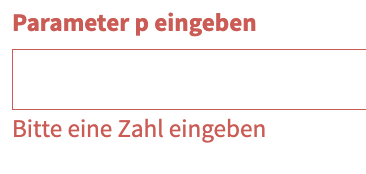
\includegraphics[width=\linewidth]{fehler.png}
    \captionof{figure}{Beispiel der Fehlermeldung}
    \label{fig:fehler}
\end{minipage}
\hfill
\begin{minipage}[t]{0.5\textwidth}
    \centering
    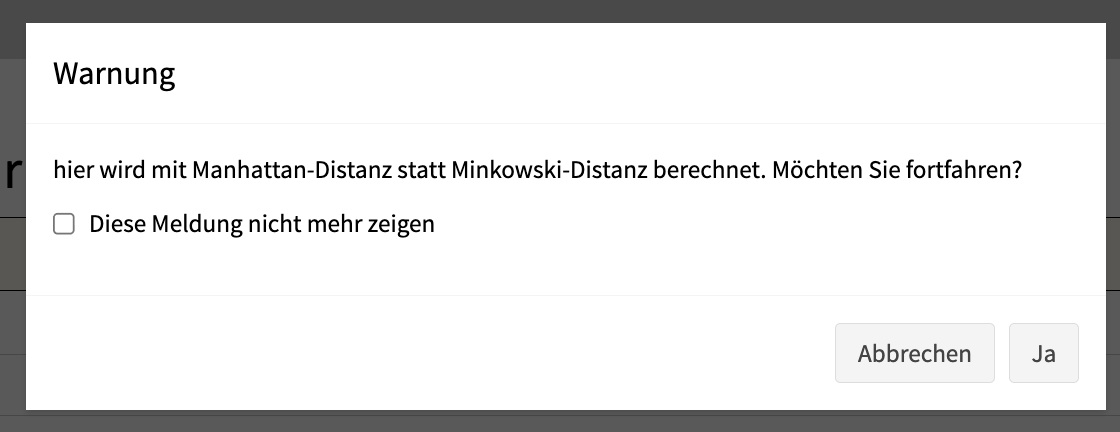
\includegraphics[width=\linewidth]{modal.png}
    \captionof{figure}{Beispiel der Pop-up-box}
    \label{fig:modal}
\end{minipage}
\end{center}



\subsection{Herausforderungen}
Die größte Herausforderung kam am meisten von den Anpassungen an alle Backend-Funktionen der verschiedenen Teams. Da wurden bis Ende viele Änderungen an den Visualisierungsfunktionen gemacht, und die mussten immer wieder angepasst und in Shiny geändert werden. Zweitens war eine der größten Herausforderungen nämlich das Debugging von vielen Abläufen in Shiny. Das war am Anfang eher problematisch, weil Shiny die Fehlermeldungen von Code nicht eindeutig zeigt, ohne Debugging-Codes selber zu erstellen. Zusätzlich war es am Anfang schwierig zu verstehen, wie Shiny überhaupt funktioniert, aber durch Videos und Demonstrationen der Shiny-Website wurde diese Herausforderung auch überwunden. Jedoch konnten durch Testen und schrittweise Anpassungen viele von diesen Problemen behoben werden. 

% etc...

\newpage
\pagestyle{fancy}
\fancyhead{}
\fancyhead[L]{Johanna}
\subsection{Farben}

\newpage
\fancyhead[L]{Adrika}
\bibliographystyle{plain}
\bibliography{Adrika-ref}

\end{document}
